%
% einleitung.tex -- Beispiel-File für die Einleitung
%
% (c) 2020 Prof Dr Andreas Müller, Hochschule Rapperswil
%
\section{Gradient Descent\label{cg:section:steepest_descent}}
\rhead{Gradient Descent}

Um den CG-Algorithmus zu verstehen, ist es hilfreich zuerst die Gradient Descent Methode zu analysieren.
Gradient Descent ist eine bekannte Methode um iterativ ein Minimierungsproblem zu lösen.
Dabei wird immer eine gewisse Schrittweite weit entlang des Gradienten des Minimierungsproblems abgestiegen.
Eine Darstellung von einem 2-dimensionalen Minimierungsproblem mit Gradient Descent findet sich in Abbildung \ref{cg:abb:steepest_descent}.

\begin{figure}	
	\centering
	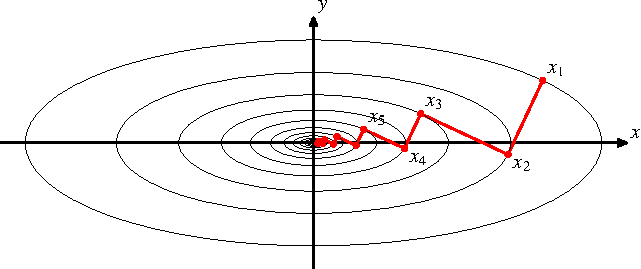
\includegraphics{papers/cg/images/descent-1}
	\caption{Gradient Descent für ellipsenförmige Niveaulinien (schlechte Konditionierung) in 2D. 
		Abbildung aus dem Seminar Buch von 2014 \cite{cg:book:hpc}.}
	\label{cg:abb:steepest_descent}
\end{figure}

\subsection{Minimierungsproblem \label{cg:subsection:Minimierungsproblem}}

Eine Lösung für $x$ kann durch Minimieren von
\begin{equation}
\Phi(x) = \frac{1}{2} x^T A x - x^T b
\end{equation}
gefunden werden.
Der folgende Beweis zeigt, wieso dies ein sinnvoller Ansatz ist.

\begin{proof}[Beweis]
	Wir definieren eine zweite Variable $z = x + \lambda y$, was uns erlaubt die folgende Differenz auszurechnen
	\begin{align}
	\Phi(z) - \Phi(x) 
	&= 
	\frac{1}{2} \left(x + \lambda y\right) ^T A \left(x + \lambda y\right)  - \left(x + \lambda y\right) ^T b
	- 
	\frac{1}{2} x^T A x + x^T b 
	\\
	&= 
	\frac{1}{2} \left(x^T A x + x^T A \lambda y + \lambda y^T A x + \lambda y^T A \lambda y\right) 
	-
	x^T b - \lambda y^T b
	- 
	\frac{1}{2} x^T A x + x^T b .	
	\end{align}
	Da $A$ symmetrisch ist, können die Terme $x^T A \lambda y$ und $\lambda y^T A x$ zusammengefasst werden (analog zur binomischen Formel)
	\begin{align}
	\Phi(z) - \Phi(x) 
	&= 
	\frac{1}{2}\cancel{ x^T A x} + x^T A \lambda y + \frac{1}{2} \lambda y^T A \lambda y
	-
	\bcancel{x^T b} - \lambda y^T b
	- 
	\frac{1}{2}\cancel{ x^T A x} + \bcancel{x^T b} \\
	&=
	\lambda x^T A y	+ \frac{1}{2} {\lambda}^2 y^T A y - \lambda y^T b \\
	&=
	\frac{{\lambda}^2}{2} y^T A y + \lambda y^T \left(Ax -b \right) .
	\end{align}
	Nun können wir den Beweis führen, indem wir $\Phi(z) \ge \Phi(x)$ setzen (da $\Phi(x)$ ja minimiert wird)
	\begin{align}
	\Phi(z) &\ge \Phi(x) 
	\\
	\Phi(z) &= \frac{{\lambda}^2}{2} y^T A y + \lambda y^T \left(Ax -b \right) + \Phi(x) 
	\\
	0 &\le \frac{{\lambda}^2}{2} y^T A y + \lambda y^T \left(Ax - b \right) \quad \forall \quad y \in \mathbb{R}^N  .
	\end{align}
	Der erste Term ist dabei quadratisch in $\lambda$, $A$ ist positiv definit und somit ist immer $\frac{{\lambda}^2}{2} y^T A y \ge 0$.
	Beim zweiten Term ist diese Bedingung nur erfüllt für alle $y$, wenn $Ax - b = 0$.
	Damit ist bewiesen, dass eine Lösung für die Gleichung $Ax = b$ durch Minimierung von $\Phi(x)$ gefunden wird.
\end{proof}

\subsection{Berechnung der Schrittweite \label{cg:subsection:schrittweite}}
Falls eine Suchrichtung gegeben ist, kann die optimale Schrittweite bestimmt werden um $\Phi(x)$ minimal werden zu lassen.
Gegeben: 
\begin{itemize}
	\item Aktueller Index $k$
	\item Suchrichtung $d_k$
	\item Startpunkt $x_k$
\end{itemize}
Wir suchen nun die optimale Schrittweite $\alpha$, um möglichst nahe an die Lösung zu kommen in der gegebenen Suchrichtung.
Dazu stellen wir wieder ein Minimierungsproblem auf
\begin{equation}
	\Phi(x_k + \alpha d_k) 
	= 
	\frac{1}{2} x_k^T A x_k + \alpha x_k^T A d_k + \frac{1}{2} {\alpha}^2 d_k^T A d_k
	-
	x_k^T b - \alpha d_k^T b .
\end{equation}
In $\alpha$ haben wir hier eine quadratische Gleichung, welche einer nach oben geöffneten Parabel entspricht (da $d_k^T A d_k \ge 0$).
Somit ist es möglich ein klares Minimum zu finden, indem wir die Gleichung nach $\alpha$ ableiten und null setzen:
\begin{equation}
	\frac{\partial \Phi(x_k + \alpha d_k) }{\partial \alpha}
	= 
	x_k^T A d_k + \alpha  d_k^T A d_k - d_k^T b
	=
	0 .
\end{equation}
Dies ergibt für $\alpha$ 
\begin{equation}
	\alpha
	= 
	\frac{d_k^T b - x_k^T A d_k}{d_k^T A d_k}
	=
	\frac{d_k^T \left(b - A x_k\right)}{d_k^T A d_k}.
\end{equation}
Wenn wir nun den Fehler der momentanen Approximation als Residuum $r_k = b - A x_k$ bezeichnen erhalten wir
\begin{equation}
	\alpha
	= 
	\frac{\langle d_k , r_k \rangle}{\langle d_k , d_k \rangle_A},
\end{equation}
wobei $\langle d_k , d_k \rangle_A = d_k^T A d_k$ das verallgemeinerte Skalarprodukt zu $A$ darstellt.
Somit haben wir nun die optimale Schrittlänge gefunden.

Daraus lässt sich nun der nächste Punkt $x_{k+1}$ berechnen als
\begin{equation}
	x_{k+1} = x_k + \frac{\langle d_k , r_k \rangle}{\langle d_k , d_k \rangle_A} d_k.
\end{equation}

\subsection{Berechnung des Gradienten}
Die neue Suchrichtung $d_{k+1}$ entspricht dem negativen Gradienten von $\Phi(x_{k+1})$.
Dieser Gradient lässt sich berechnen als
\begin{equation}
	d_{k+1} = - \nabla \Phi(x_{k+1}) = - \nabla \frac{1}{2} x_{k+1}^T A x_{k+1} - x_{k+1}^T b = -(Ax_{k+1} - b) = b - Ax_{k+1}.
\end{equation}
Somit ist die neue Abstiegsrichtung identisch zum neuen Residuum $r_{k+1}$.

\subsection{Probleme beim Gradient Descent}
Mit den hier hergeleiteten Resultaten kann eine approximative Lösung gefunden werden.
Die Konvergenzgeschwindigkeit ist allerdings stark abhängig von der Form von $A$.
Das Beispiel in Abbildung \ref{cg:abb:steepest_descent} zeigt (in 2D), wie Gradient Descent bei ovalen Niveaulinien zu oszillieren beginnt.
Die Konvergenz ist also in diesem Fall sehr langsam, die exakte Lösung wird nie erreicht.
Falls die Niveaulinien allerdings eher rund sind, erhöht sich die Konvergenzgeschwindigkeit.

Diese Probleme werden mit der Erweiterung zum CG-Algorithmus behoben.

\subsection{Beispiel zur Motivation der $A$-Orthogonalität} \label{cg:subsec:aortho}
Das folgende Beispiel soll ausgehend von Gradient Descent die Motivation liefern, weshalb im CG-Algorithmus die $A$-Orthogonalität wichtig ist.
Unter $A$-Orthogonalität ($\perp_A$) versteht man, dass das verallgemeinerte Skalarprodukt von $A$ verschwindet:
\begin{equation}
	a \perp_A b \Longrightarrow a^T A b = \langle a , b \rangle_A = 0.
\end{equation}
Richtungen welche $A$-orthogonal stehen, werden auch konjugiert bezüglich $A$ genannt.
Dies erklärt den Namen des CG-Verfahrens.
Für das Beispiel definieren wir $A$, $b$, $x_1$ und berechnen $x_2$:
\begin{align}\nonumber
	A 	&= 		\begin{pmatrix}
				4 & 0\\
				0 & 9 
				\end{pmatrix} \nonumber\\
	b 	&= 		\begin{pmatrix}
				0\\
				0
				\end{pmatrix} \nonumber\\
	x_1 &= 		\begin{pmatrix}
				1\\
				1
				\end{pmatrix} \nonumber\\
	r_1	&= 		b - A x_1 = - 	\begin{pmatrix}
								4\\
								9
								\end{pmatrix} \nonumber\\
	d_1 &= r_1 \nonumber\\
	x_2 &= x_1 + \frac{\langle r_1 , r_1 \rangle}{\langle r_1 , r_1 \rangle_A} r_1 = 	\begin{pmatrix}
																						0.51\\
																						-0.1
																						\end{pmatrix}. \\
\end{align}
Dieses Gleichungssystem ist gelöst im Ursprung $x = \begin{pmatrix}0\\0\end{pmatrix}$.
Um im nächsten Schritt eine Lösung finden zu können, müsste die nächste Abstiegsrichtung dem Vektor von $x_2$ zum Ursprung entsprechen.
Wenn wir das $A$-Skalarprodukt von $-x_2$ und $d_1$ berechnen, verschwindet dieses:
\begin{equation}
	\langle -x_2 , d_1 \rangle_A = 	-x_2^T A d_1 = 
		\begin{pmatrix} 0.51 & -0.1 \end{pmatrix} 
		\begin{pmatrix} 4 & 0\\
						0 & 9 
		\end{pmatrix} 
		\begin{pmatrix} -4\\
						-9 
		\end{pmatrix} = 0 \nonumber
\end{equation}
was der $A$-Orthogonalität entspricht.
Damit ist gezeigt, dass die optimale zweite Abstiegsrichtung $A$-orthogonal zur ersten Abstiegsrichtung wäre.
Also ist $A$-Orthogonalität das entscheidende Konzept um dem CG-Algorithmus zu ermöglichen in $N$-Schritten eine exakte Lösung zu finden.